%%%%%%%%%%%%%%%%%%%%%%%%%%%%%%%%%%%%%%%%%%%%%%%%%%%%%%
% A Beamer template for University of Wollongong     %
% Based on THU beamer theme                          %
% Author: Qiuyu Lu                                   %
% Date: July 2024                                    %
% LPPL Licensed.                                     %
%%%%%%%%%%%%%%%%%%%%%%%%%%%%%%%%%%%%%%%%%%%%%%%%%%%%%%

\documentclass[serif, aspectratio=169]{beamer}
%\documentclass[serif]{beamer}  % for 4:3 ratio
\usepackage[T1]{fontenc} 
\usepackage{fourier} % see "http://faq.ktug.org/wiki/uploads/MathFonts.pdf" for other options
\usepackage{hyperref}
% \hypersetup{
%   colorlinks   = true,    % Colours links instead of ugly boxes
%   urlcolor     = blue,    % Colour for external hyperlinks
%   linkcolor    = blue,    % Colour of internal links
% %   citecolor    = red      % Colour of citations
% }
\usepackage{latexsym,amsmath,xcolor,multicol,booktabs,calligra}
\usepackage{graphicx,pstricks,listings,stackengine}
\usepackage{lipsum}

\author[Danko, Strygin]{Danila Danko, MS-SE \inst{1} \and Nikita Strygin, MS-SE \inst{1} \and \newline \newline {Supervisor: Nikolai Kudasov \inst{1}}}
\title{Query-Driven Language Server Architecture using Second-Order Abstract Syntax}

\institute{
    \inst{1}Innopolis University
}
\date{\small \today}

\usepackage{styling}

% defs
\def\cmd#1{\texttt{\color{red}\footnotesize $\backslash$#1}}
\def\env#1{\texttt{\color{blue}\footnotesize #1}}
\definecolor{deepblue}{rgb}{0,0,0.5}
\definecolor{deepred}{RGB}{153,0,0}
\definecolor{deepgreen}{rgb}{0,0.5,0}
\definecolor{halfgray}{gray}{0.55}

\lstset{
    basicstyle=\ttfamily\small,
    keywordstyle=\bfseries\color{deepblue},
    emphstyle=\ttfamily\color{deepred},    % Custom highlighting style
    stringstyle=\color{deepgreen},
    numbers=left,
    numberstyle=\small\color{halfgray},
    rulesepcolor=\color{red!20!green!20!blue!20},
    frame=shadowbox,
}


\begin{document}

\begin{frame}
	\titlepage
\end{frame}

\begin{frame}
	\tableofcontents[sectionstyle=show,
		subsectionstyle=show/shaded/hide,
		subsubsectionstyle=show/shaded/hide]
\end{frame}

\section{Introduction}

\begin{frame}{Context}
	\begin{itemize}
		[<+-| alert+>] % stepwise alerts
		\item The Language Server Protocol \cite{noauthor_language_server_protocol_2024} standardized the protocol of communication between source code editors and language servers that provide language features like auto complete.
		\item There are language servers for mainstream languages such as C\#, Java, C++ \cite{lsp_implementations}. Such servers improve the developer experience by supporting the "go to definition", "lookup the type on hover", "rename all occurences" queries.
	\end{itemize}
\end{frame}

\begin{frame}{Problem}
	\begin{itemize}
		[<+-| alert+>] % stepwise alerts
		\item Multiple programming languages are implemented in Haskell \cite{github_haskell_programming_language}, \cite{hackage_formal_languages}, \cite{hackage_language}.
		\item Only a half of the GitHub repositories for programming languages implemented in Haskell provide a language server \cite{github_lsp_module}.
		      % TODO check more accurately
		\item There exist frameworks for TypeScript (\texttt{Langium}~\cite{noauthor_langium_nodate}) and Python (\texttt{lsp-tree-sitter}~\cite{noauthor_neomuttlsp-tree-sitter_2024}) that simplify integration with the LSP for new languages.
		\item However, to our best knowledge, there is no such framework for languages implemented in Haskell!
	\end{itemize}
\end{frame}

\begin{frame}{Solution}
	\begin{itemize}
		[<+-| alert+>] % stepwise alerts
		\item Language servers share some features, such as "go to definition".
		\item We assume that some of these features can be implemented in a Haskell framework that is independent of the target language (language-agnostic) for which LSP integration is developed.
		\item A promising approach is to work with the Second-Order Abstract Syntax (SOAS) \cite{fiore_formal_2022} of the target language.
		\item The main idea of SOAS is to provide a language-agnostic machinery for describing variable introduction in Abstract Syntax Tree (like lambda abstraction in Lambda calculus).
		\item This allows it to provide generic mechanisms for scope resolution ("go to definition"), variable bindings ("lookup the type on hover"), and substitution ("rename all occurences").
	\end{itemize}
\end{frame}

\section{Contribution}

\begin{frame}{Contribution}
	\begin{itemize}
		[<+-| alert+>] % stepwise alerts
		\item We want to implement in Haskell a language-agnostic framework that simplifies integration with LSP of (new) languages written in Haskell.
		\item The framework will primarily be based on the \texttt{free-foil} \cite{hackage_free_foil} (SOAS manipulation), \texttt{BNFC} \cite{hackage_bnfc} (parsing), \texttt{lsp} \cite{hackage_lsp} (library for building LSP) packages.
	\end{itemize}
\end{frame}

\section{Evaluation criteria}
\label{sec:evaluation_criteria}

\begin{frame}{Metrics}
	\begin{itemize}
		[<+-| alert+>] % stepwise alerts
		\item We plan to provide integration with LSP for Simply typed lambda calculus (STLC) \cite{wiki_stlc} and Stella Core \cite{noauthor_fizrukstella_nodate} with (Approach 1) and without (Approach 2) our framework.
		\item We will measure for both approaches and compare:
		      \begin{itemize}
			      \item The lines of code required for integration and some other complexity metrics.
			      \item The performance of the server on a large (probably generated) code base (approx.~10KLoC).
		      \end{itemize}
		\item Condition for success: metrics for the Approach 1 are at most 10\% better than metrics for the Approach 2.
	\end{itemize}
\end{frame}

\section{Plan of work}

\subsection{Review the literature}

\begin{frame}{Review the literature}
	\begin{itemize}
		\item Read papers on SOAS \cite{fiore_formal_2022}, Foil \cite{maclaurin_foil_2022} and Free foil \cite{kudasov_free_2024}.
		\item Read the \texttt{free-foil} package documentation \cite{hackage_free_foil}.
	\end{itemize}
\end{frame}

\subsection{Preliminary results}

\begin{frame}{Preliminary results}
	\begin{itemize}
		\item We created a repository \cite{github_query_driven_free_foil} for the thesis work.
		\item We implemented a parser and pretty-printer of STLC as defined in \cite{dunfield_bidirectional_2020} using BNFC.
	\end{itemize}
\end{frame}

\subsection{Practice with Free Foil}

\begin{frame}{Practice with Free Foil}
	\begin{itemize}
		\item Complete exercises on AST manipulation provided by Nikolai.
		\item Complete these exercises using Free foil.
	\end{itemize}
\end{frame}

\subsection{Practice with Simply typed lambda calculus (STLC)}

\begin{frame}{Type checker and interpreter for STLC}
	\begin{itemize}
		\item Implement a type checker and interpreter for STLC.
		\item Features:
		      \begin{itemize}
			      \item Single module on the input and the output.
			      \item Use BNFC for parsing and pretty-printing.
			      \item Use Free Foil and Template Haskell.
			      \item Show error location in the code.
		      \end{itemize}
	\end{itemize}

\end{frame}

\begin{frame}{Language server for STLC}
	\begin{itemize}
		\item Implement a language server and a simple VS Code extension for STLC.
		\item Use the \texttt{lsp} \cite{hackage_lsp} package.
		\item Features:
		      \begin{itemize}
			      \item Go to definition.
			      \item Type on hover.
			      \item Maybe something else that makes sense for STLC.
		      \end{itemize}
	\end{itemize}

\end{frame}

\subsection{Practice with Stella Core}

\begin{frame}{Type checker and interpreter for Stella Core}
	\begin{itemize}
		\item Implement a type checker and interpreter for Stella Core.
		\item Features:
		      \begin{itemize}
			      \item Single module on the input and the output.
			      \item Use BNFC for parsing and pretty-printing.
			      \item Use Free Foil and Template Haskell.
			      \item Show error location in the code.
		      \end{itemize}
	\end{itemize}

\end{frame}

\begin{frame}{Language server for Stella Core}
	\begin{itemize}
		\item Implement a language server, and a simple VS Code extension for Stella Core.
		\item Use the \texttt{lsp} \cite{hackage_lsp} package.
		\item Features:
		      \begin{itemize}
			      \item Type and documentation on hover.
			      \item Autocompletion.
			      \item Inlay (type) hints.
			      \item (Un)folding scopes.
			      \item InfoView - a separate panel that shows context (what is in scope, the type of the current expression or goal)
			      \item Something else.
		      \end{itemize}
	\end{itemize}

\end{frame}

\subsection{Evaluate the results}

\begin{frame}{Evaluation}
	\begin{itemize}
		\item Generate large code bases (approx. 10KLoC) for STLC and Stella.
		\item Evaluate the results using the \hyperlink{sec:evaluation_criteria}{Evaluation criteria}.
	\end{itemize}

\end{frame}


% \section{Literature Review}

% \subsection{GPT3-derived Models DALLE \& CLIP}

% \begin{frame}
%     \begin{itemize}
%         \item \lipsum[2][1-4]
%         \item \lipsum[2][5-9]
%         \item Results accessible at \newline \url{https://scholar.google.com}
%     \end{itemize}
% \end{frame}


% \section{Methods}

% \subsection{Diffusion Model}

% \begin{frame}{Title}
%     \begin{itemize}
%         \item \lipsum[3][1-4]
%     \end{itemize}
%     \begin{table}[h]
%         \centering
%         \begin{tabular}{c|c}
%             Microsoft\textsuperscript{\textregistered}  Windows & Apple\textsuperscript{\textregistered}  Mac OS \\
%             \hline
%             Windows-Kernel & Unix-like \\
%             Arm, Intel & Intel, Apple Silicon \\
%             Sudden update & Stable update \\
%             Less security & More security \\
%             ... & ... \\
%         \end{tabular}
%     \end{table}
% \end{frame}

% \begin{frame}{Algorithms}
%     \begin{exampleblock}{Non-Numbering Formula}
%         \begin{equation*}
%             J(\theta) = \mathbb{E}_{\pi_\theta}[G_t] = \sum_{s\in\mathcal{S}} d^\pi (s)V^\pi(s)=\sum_{s\in\mathcal{S}} d^\pi(s)\sum_{a\in\mathcal{A}}\pi_\theta(a|s)Q^\pi(s,a)
%         \end{equation*}
%     \end{exampleblock}
%     \begin{exampleblock}{Multi-Row Formula\footnote{If text appears in the formula, use $\backslash$mathrm\{\} or $\backslash$text\{\} instead}}
%         \begin{align}
%             Q_\mathrm{target}&=r+\gamma Q^\pi(s^\prime, \pi_\theta(s^\prime)+\epsilon)\\
%             \epsilon&\sim\mathrm{clip}(\mathcal{N}(0, \sigma), -c, c)\nonumber
%         \end{align}
%     \end{exampleblock}
% \end{frame}

% \begin{frame}
%     \begin{exampleblock}{Numbered Multi-line Formula}
%         % Taken from Mathmode.tex
%         \begin{multline}
%             A=\lim_{n\rightarrow\infty}\Delta x\left(a^{2}+\left(a^{2}+2a\Delta x+\left(\Delta x\right)^{2}\right)\right.\label{eq:reset}\\
%             +\left(a^{2}+2\cdot2a\Delta x+2^{2}\left(\Delta x\right)^{2}\right)\\
%             +\left(a^{2}+2\cdot3a\Delta x+3^{2}\left(\Delta x\right)^{2}\right)\\
%             +\ldots\\
%             \left.+\left(a^{2}+2\cdot(n-1)a\Delta x+(n-1)^{2}\left(\Delta x\right)^{2}\right)\right)\\
%             =\frac{1}{3}\left(b^{3}-a^{3}\right)
%         \end{multline}
%     \end{exampleblock}
% \end{frame}

% \begin{frame}{Graphics and Columns}
%     \begin{minipage}[c]{0.3\linewidth}
%         \psset{unit=0.8cm}
%         \begin{pspicture}(-1.75,-3)(3.25,4)
%             \psline[linewidth=0.25pt](0,0)(0,4)
%             \rput[tl]{0}(0.2,2){$\vec e_z$}
%             \rput[tr]{0}(-0.9,1.4){$\vec e$}
%             \rput[tl]{0}(2.8,-1.1){$\vec C_{ptm{ext}}$}
%             \rput[br]{0}(-0.3,2.1){$\theta$}
%             \rput{25}(0,0){%
%             \psframe[fillstyle=solid,fillcolor=lightgray,linewidth=.8pt](-0.1,-3.2)(0.1,0)}
%             \rput{25}(0,0){%
%             \psellipse[fillstyle=solid,fillcolor=yellow,linewidth=3pt](0,0)(1.5,0.5)}
%             \rput{25}(0,0){%
%             \psframe[fillstyle=solid,fillcolor=lightgray,linewidth=.8pt](-0.1,0)(0.1,3.2)}
%             \rput{25}(0,0){\psline[linecolor=red,linewidth=1.5pt]{->}(0,0)(0.,2)}
% %           \psRotation{0}(0,3.5){$\dot\phi$}
% %           \psRotation{25}(-1.2,2.6){$\dot\psi$}
%             \psline[linecolor=red,linewidth=1.25pt]{->}(0,0)(0,2)
%             \psline[linecolor=red,linewidth=1.25pt]{->}(0,0)(3,-1)
%             \psline[linecolor=red,linewidth=1.25pt]{->}(0,0)(2.85,-0.95)
%             \psarc{->}{2.1}{90}{112.5}
%             \rput[bl](.1,.01){C}
%         \end{pspicture}
%     \end{minipage}\hspace{2cm}
%     \begin{minipage}{0.5\linewidth}
%         \medskip
%         % \hspace{2cm}
%         \begin{figure}[h]
%             \centering
%             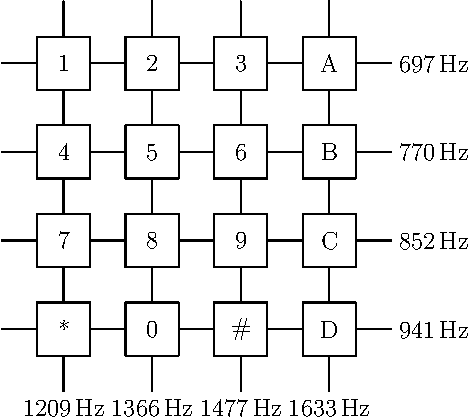
\includegraphics[height=.4\textheight]{pic/sample.pdf}
%         \end{figure}
%     \end{minipage}
% \end{frame}

% \begin{frame}[fragile]{\LaTeX{} Common Commands}
%     \begin{exampleblock}{Commands}
%         \centering
%         \footnotesize
%         \begin{tabular}{llll}
%             \cmd{chapter} & \cmd{section} & \cmd{subsection} & \cmd{paragraph} \\
%             chapter & section & sub-section & paragraph \\\hline
%             \cmd{centering} & \cmd{emph} & \cmd{verb} & \cmd{url} \\
%             center & emphasize & original & hyperlink \\\hline
%             \cmd{footnote} & \cmd{item} & \cmd{caption} & \cmd{includegraphics} \\
%             footnote & list item & caption & insert image \\\hline
%             \cmd{label} & \cmd{cite} & \cmd{ref} \\
%             label & citation & refer\\\hline
%         \end{tabular}
%     \end{exampleblock}
%     \begin{exampleblock}{Environment}
%         \centering
%         \footnotesize
%         \begin{tabular}{lll}
%             \env{table} & \env{figure} & \env{equation}\\
%             table & figure & formula \\\hline
%             \env{itemize} & \env{enumerate} & \env{description}\\
%             non-numbering item & numbering item & description \\\hline
%         \end{tabular}
%     \end{exampleblock}
% \end{frame}

% \begin{frame}[fragile]{\LaTeX{} Examples of environmental commands}
%     \begin{minipage}{0.5\linewidth}
% \begin{lstlisting}[language=TeX]
% \begin{itemize}
%   \item A \item B
%   \item C
%   \begin{itemize}
%     \item C-1
%   \end{itemize}
% \end{itemize}
% \end{lstlisting}
%     \end{minipage}\hspace{1cm}
%     \begin{minipage}{0.3\linewidth}
%         \begin{itemize}
%             \item A
%             \item B
%             \item C
%             \begin{itemize}
%                 \item C-1
%             \end{itemize}
%         \end{itemize}
%     \end{minipage}
%     \medskip
%     \pause
%     \begin{minipage}{0.5\linewidth}
% \begin{lstlisting}[language=TeX]
% \begin{enumerate}
%   \item A \item B
%   \item C
%   \begin{itemize}
%     \item[n+e]
%   \end{itemize}
% \end{enumerate}
% \end{lstlisting}
%     \end{minipage}\hspace{1cm}
%     \begin{minipage}{0.3\linewidth}
%         \begin{enumerate}
%             \item A
%             \item B
%             \item C
%             \begin{itemize}
%                 \item[n+e]
%             \end{itemize}
%         \end{enumerate}
%     \end{minipage}
% \end{frame}

% \begin{frame}[fragile]{\LaTeX{} Formulas}
%     \begin{columns}
%         \begin{column}{.55\textwidth}
% \begin{lstlisting}[language=TeX]
% $V = \frac{4}{3}\pi r^3$

% \[
%   V = \frac{4}{3}\pi r^3
% \]

% \begin{equation}
%   \label{eq:vsphere}
%   V = \frac{4}{3}\pi r^3
% \end{equation}
% \end{lstlisting}
%         \end{column}
%         \begin{column}{.4\textwidth}
%             $V = \frac{4}{3}\pi r^3$
%             \[
%                 V = \frac{4}{3}\pi r^3
%             \]
%             \begin{equation}
%                 \label{eq:vsphere}
%                 V = \frac{4}{3}\pi r^3
%             \end{equation}
%         \end{column}
%     \end{columns}
%     \begin{itemize}
%         \item more information \href{https://ja.overleaf.com/learn/latex/Mathematical_expressions}{\color{purple}{here}}
%     \end{itemize}
% \end{frame}

% \begin{frame}[fragile]
%     \begin{columns}
%         \column{.6\textwidth}
% \begin{lstlisting}[language=TeX]
% \begin{table}[htbp]
%   \caption{numbers & meaning}
%   \label{tab:number}
%   \centering
%   \begin{tabular}{cl}
%     \toprule
%     number & meaning \\
%     \midrule
%     1 & 4.0 \\
%     2 & 3.7 \\
%     \bottomrule
%   \end{tabular}
% \end{table}
% \end{lstlisting}
%         \column{.4\textwidth}
%         \begin{table}[htpb]
%             \centering
%             \caption{numbers \& meaning}
%             \label{tab:number}
%             \begin{tabular}{cl}\toprule
%                 numbers & meaning \\\midrule
%                 1 & 4.0\\
%                 2 & 3.7\\\bottomrule
%             \end{tabular}
%         \end{table}
%         \normalsize formula~(\ref{eq:vsphere}) at previous slide and Table~\ref{tab:number}.
%     \end{columns}
% \end{frame}

% \section{Results}
% \begin{frame}
%     \begin{itemize}
%         \item \lipsum[4][1-4]
%         \item \lipsum[4][5-9]
%         \item \lipsum[5][1-4]
%         \item \lipsum[5][5-8]
%     \end{itemize}
% \end{frame}

\section{References}

\begin{frame}[allowframebreaks]
	\bibliography{ref}
	\bibliographystyle{ieeetr}
	% \nocite{*} % used here because no citation happens in slides
	% if there are too many try use:
	% \tiny\bibliographystyle{alpha}
\end{frame}


\begin{frame}
	\begin{center}
		{\Huge Thank You}
	\end{center}
\end{frame}

\end{document}